% ===== SLIDE: Architecture Overview =====
\begin{frame}{STMN Architecture Overview}
    The STMN framework processes video sequences using a modified ResNet-50 backbone, enhanced with two novel memory modules:
    
    \smallskip
    \begin{columns}[T]
    \column{0.48\textwidth}
        \begin{block}{\centering Spatial Memory Module (SMM)}
            \small\centering
            Operates at the frame level to refine spatial features by minimizing the influence of moving distractors.
        \end{block}
    \column{0.48\textwidth}
        \begin{block}{\centering Temporal Memory Module (TMM)}
            \small\centering
            Operates at the sequence level to aggregate refined spatial features into a robust, unified identity representation.
        \end{block}
    \end{columns}

    \vspace{0.5em}
    \begin{alertblock}{Information Flow}
        \small
        Raw Video Tracklet $\rightarrow$ ResNet-50 Features $\rightarrow$ \textbf{SMM} (Spatial Refinement) $\rightarrow$ \textbf{TMM} (Temporal Aggregation) $\rightarrow$ Final Feature Descriptor
    \end{alertblock}
\end{frame}

% ===== SLIDE: The Problem of Distractors =====
\begin{frame}{The Challenge of Moving Distractors}
    \centering
    \IfFileExists{images/example_noise.png}{
        
\includegraphics[width=0.8\textwidth]{images/example_noise.png}
    }{
        \IfFileExists{example_noise.png}{
            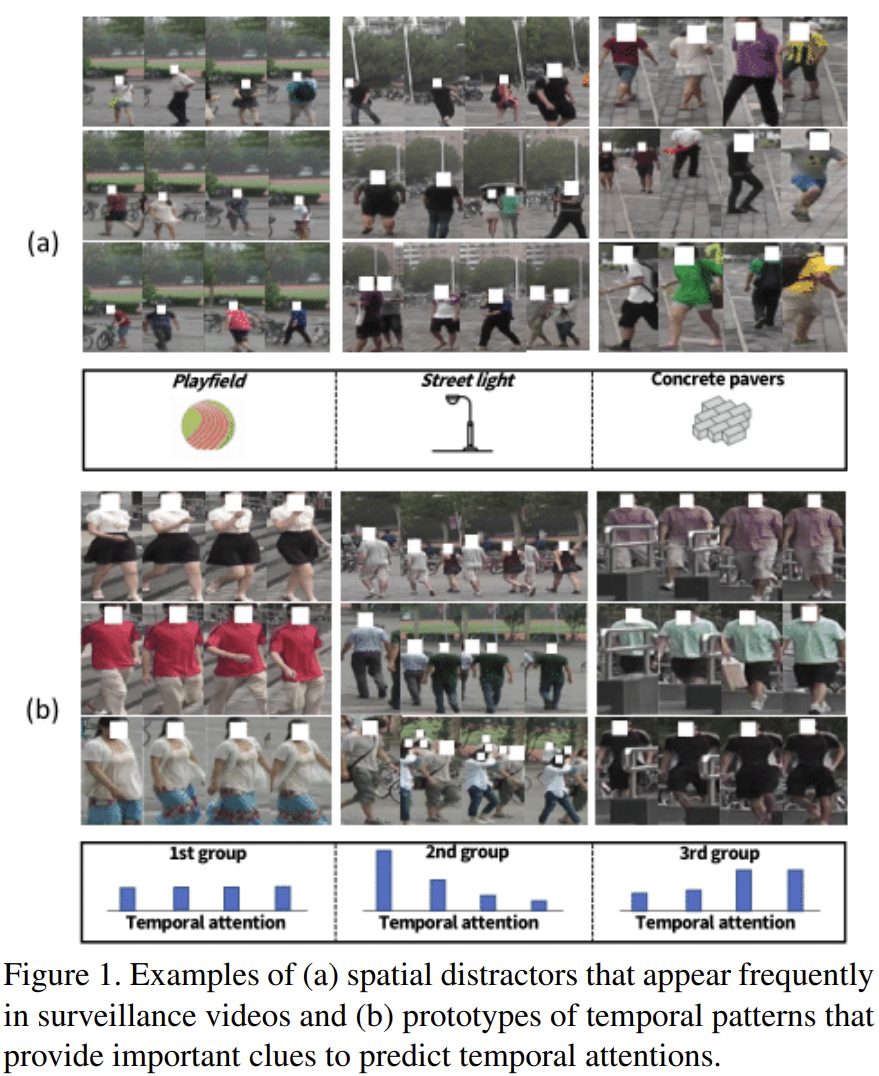
\includegraphics[width=0.8\textwidth]{example_noise.png}
        }{
            \textit{(Distractor Example Image Missing)}
        }
    }

    \smallskip
    \small 
    \textbf{Example:} The target person (red box) is heavily occluded by a moving bicycle (blue box) across multiple frames. Standard optical flow interprets the bicycle as the primary motion, confusing the model.
\end{frame}

% ===== SLIDE: Spatial Memory Module (SMM) =====
\begin{frame}{Spatial Memory Module (SMM)}
    The SMM aims to "remember" typical background and distractor patterns to suppress them in the input features.
    
    \centering
    \IfFileExists{images/spatial_memory.png}{
        
\includegraphics[width=0.7\textwidth]{images/spatial_memory.png}
    }{
        \IfFileExists{spatial_memory.png}{
            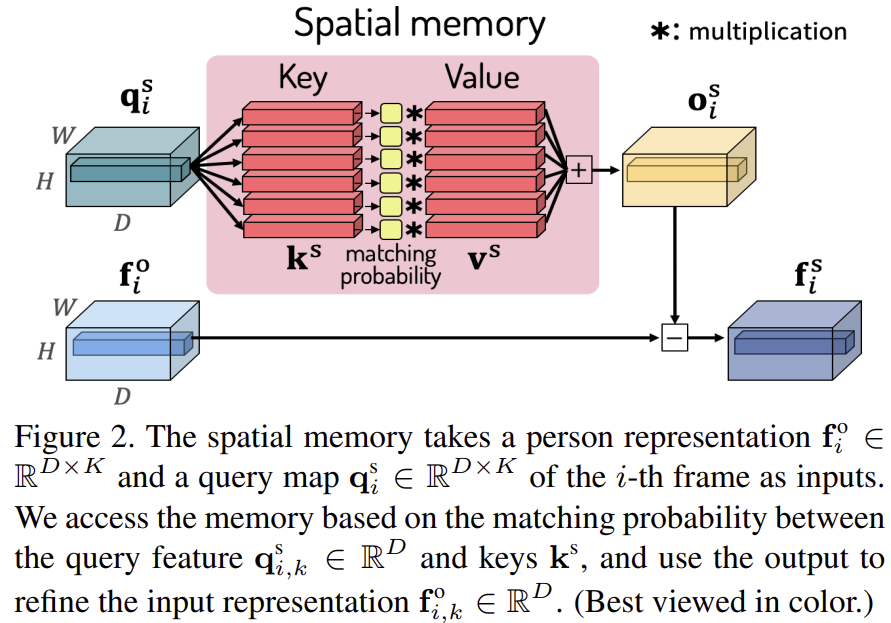
\includegraphics[width=0.7\textwidth]{spatial_memory.png}
        }{
            \textit{(Spatial Memory Architecture Image Missing)}
        }
    }

    \smallskip
    \small
    \begin{itemize}\setlength\itemsep{2pt}
        \item Consists of memory slots $M_s \in \mathbb{R}^{N_s \times C}$ storing background patterns.
        \item Calculates a match probability between input features and memory slots.
        \item Subtracts the matched background features from the input, outputting a \textbf{refined spatial feature}.
    \end{itemize}
\end{frame}

% ===== SLIDE: Temporal Memory Module (TMM) =====
\begin{frame}{Temporal Memory Module (TMM)}
    The TMM aggregates the refined spatial features from the SMM to form a single, robust sequence-level descriptor.
    
    \centering
    \IfFileExists{images/temporal_memory.png}{
        
\includegraphics[width=0.7\textwidth]{images/temporal_memory.png}
    }{
        \IfFileExists{temporal_memory.png}{
            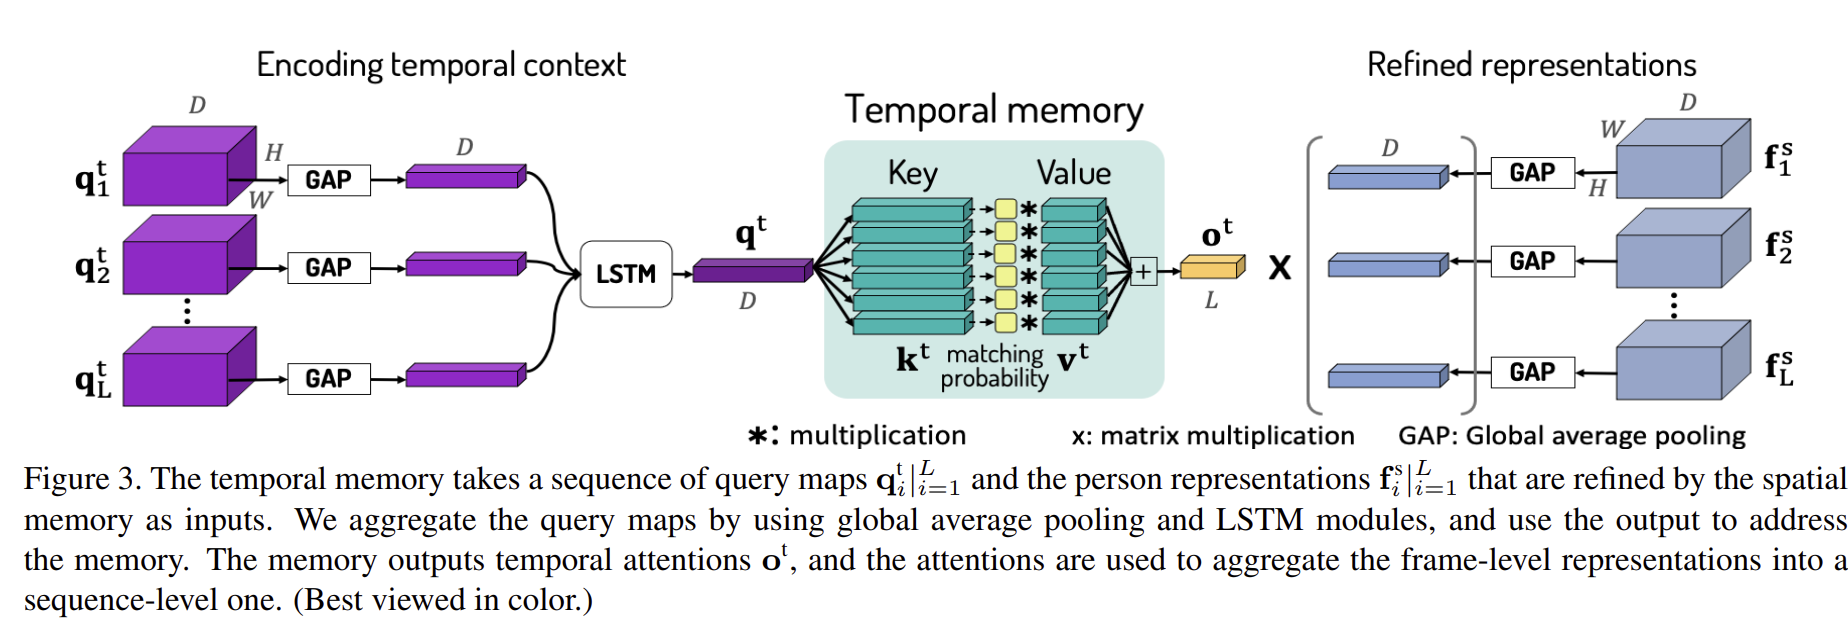
\includegraphics[width=0.7\textwidth]{temporal_memory.png}
        }{
            \textit{(Temporal Memory Architecture Image Missing)}
        }
    }

    \smallskip
    \small
    \begin{itemize}\setlength\itemsep{2pt}
        \item Consists of temporal memory slots $M_t \in \mathbb{R}^{N_t \times C}$.
        \item Input frames update the memory states sequentially using a GRU-like mechanism.
        \item Output is dynamically generated by attending to the most relevant stored temporal patterns, ignoring heavily occluded frames.
    \end{itemize}
\end{frame}